\section{主结果与适用域}
\subsection{三类股票池的回归与Rank IC}
\begingroup\small\setlength{\tabcolsep}{4pt}
\begin{table}[H]\centering
\caption*{\textbf{表C1(a)　回归法汇总}}
\begin{tabular*}{\textwidth}{@{\extracolsep{\fill}}llrrrr@{}}\toprule
股票池 & 因子 & $|t|$均值 & $|t|>2$占比 & $t$均值 & \makecell{因子收益均值\\（\%/月）} \\ \midrule
沪深300 & BP & 2.106 & 101/228 (44.30\%) & 0.531 & 0.34 \\
中证500 & BP & 1.898 & 87/228 (38.16\%) & 0.466 & 0.25 \\
全部 A 股 & BP & 4.729 & 160/228 (70.18\%) & 1.757 & 0.40 \\
\bottomrule\end{tabular*}
\par\smallskip\raggedright\footnotesize 各池均有228期。回归系数对应一单位标准化BP暴露；表中是截面$t$统计量。\end{table}
\endgroup

三池的平均回归系数均为正。全部 A 股绝对t均值4.729，绝对t>2共160/228期，t均值1.757；沪深300、中证500的t均值分别为0.531和0.466。全部 A 股t>2为100期、t<$-$2为60期，WLS系数为正的月份为126/228，少于下表中IC为正的162/228，排序证据的逐月一致性强于线性回归证据。

\begingroup\small\setlength{\tabcolsep}{4pt}
\begin{table}[H]\centering
\caption*{\textbf{表C1(b)　Rank IC汇总}}
\begin{tabular*}{\textwidth}{@{\extracolsep{\fill}}llrrrr@{}}\toprule
股票池 & 因子 & IC均值 & IC标准差 & ICIR & $IC>0$占比 \\ \midrule
沪深300 & BP & 0.0366 & 0.1279 & 0.286 & 134/228 (58.77\%) \\
中证500 & BP & 0.0350 & 0.1056 & 0.332 & 145/228 (63.60\%) \\
全部 A 股 & BP & 0.0566 & 0.1028 & 0.550 & 162/228 (71.05\%) \\
\bottomrule\end{tabular*}
\par\smallskip\raggedright\footnotesize 时间序列标准差使用$n-1$分母；ICIR未年化。\end{table}
\endgroup

全部 A 股平均Rank IC为0.0566，162/228期为正，ICIR为0.550；沪深300与中证500分别为0.0366、0.0350。三池方向与平均回归系数一致，全部 A 股的强度最高。三池使用同一窗口，强度差异来自股票池的成员范围与截面规模。

\subsection{五层排序与多空收益}
\begingroup\small\setlength{\tabcolsep}{4pt}
\begin{table}[H]\centering
\caption*{\textbf{表C2(a)　五层年化净收益}}
\begin{tabular*}{\textwidth}{@{\extracolsep{\fill}}llrrrrrr@{}}\toprule
股票池 & 因子 & Q1 & Q2 & Q3 & Q4 & Q5 & \makecell{递增相邻\\层数/4} \\ \midrule
沪深300 & BP & 2.22 & 3.78 & 3.14 & 7.31 & 10.40 & 3/4 \\
中证500 & BP & 5.64 & 7.61 & 8.99 & 10.16 & 13.50 & 4/4 \\
全部 A 股 & BP & 4.55 & 8.71 & 14.00 & 17.75 & 20.98 & 4/4 \\
\bottomrule\end{tabular*}
\par\smallskip\raggedright\footnotesize 收益单位为\%，为复合年化净收益（CAGR）。三池层序与年化收益的Spearman相关分别为0.900、1.000、1.000。每池228期，所有层均已扣教材成本。\end{table}
\endgroup

全部 A 股五层年化净收益从4.55\%依次升至20.98\%，4/4个相邻层递增，层序与年化收益Spearman为1，呈严格单调。中证500同样4/4递增；沪深300为3/4，仅Q3略低于Q2。三池排序均支持正向BP假说。成本拖累很小：建仓后Q1、Q5的平均月度只数换手为13.6\%与11.4\%，按双边千分之四折合年化约0.65与0.55个百分点；中间三层换手较高，为24.4\%至28.7\%。

\begingroup\small\setlength{\tabcolsep}{4pt}
\begin{table}[H]\centering
\caption*{\textbf{表C2(b)　多空绩效与多头超额}}
\begin{tabular*}{\textwidth}{@{\extracolsep{\fill}}lrrrrr@{}}\toprule
股票池 & \makecell{多空年化\\（\%）} & 夏普 & \makecell{最大回撤\\（\%）} & 多空月胜率 & \makecell{Q5年化超额\\（百分点）} \\ \midrule
沪深300 & 5.28 & 0.470 & -47.50 & 121/228 (53.07\%) & 3.41 \\
中证500 & 5.09 & 0.513 & -22.94 & 121/228 (53.07\%) & 2.79 \\
全部 A 股 & 13.00 & 1.150 & -15.66 & 136/228 (59.65\%) & 5.31 \\
\bottomrule\end{tabular*}
\par\smallskip\raggedright\footnotesize 夏普、回撤和胜率对应多空；Q5年化超额为相对内部等权毛基准的算术年化差额。\end{table}
\endgroup

全部 A 股扣双腿成本后的多空年化为13.00\%、夏普1.150、最大回撤$-$15.66\%。两个指数股票池多空年化约5\%，回撤更深：沪深300为$-$47.50\%（2018-12至2021-07），中证500为$-$22.94\%（2018-10至2021-06），都对应下文2019至2021年的失效期。按第3.2节的分解，全部 A 股多空净收益的算术年化值为12.89个百分点，其中多头部分5.31个百分点、空头部分7.59个百分点，低BP端的落后贡献约59\%。

\Needspace{70mm}
\subsection{排序关联与线性系数的时间路径}
\begin{figure}[H]\centering
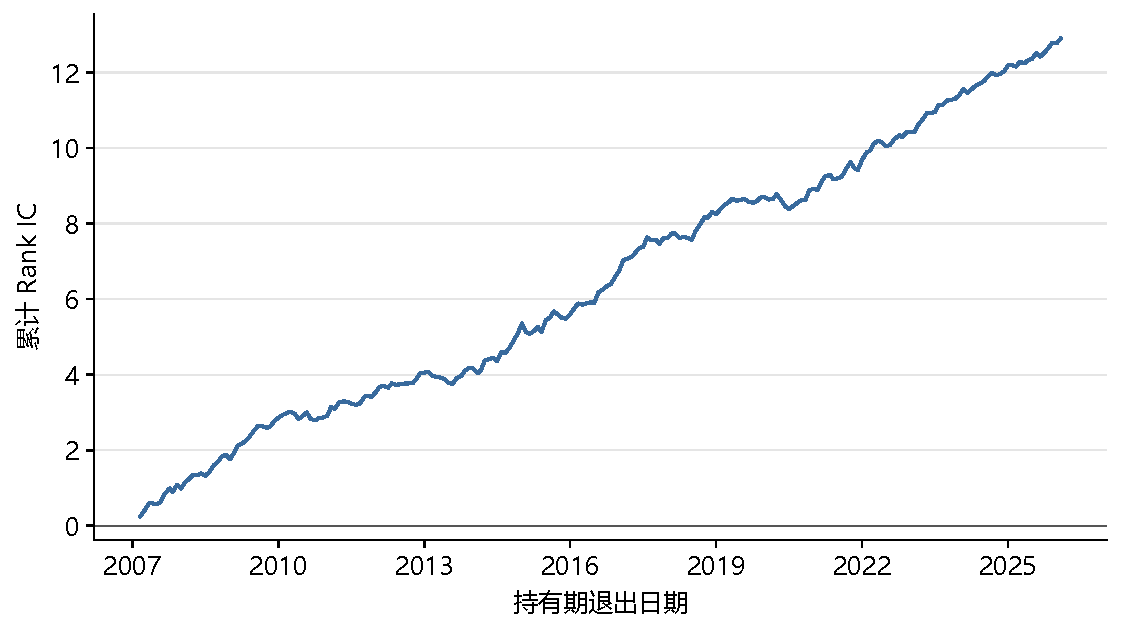
\includegraphics{figures/D2.pdf}
\caption*{\textbf{图D2　Rank IC算术累计}\ 全部 A 股，228期；逐期相加，纵轴是Rank IC算术累计。横轴为持有期归属月份。}
\end{figure}

三个日历块的平均Rank IC分别为0.0502（2007-02至2013-12，83期）、0.0567（2014-01至2020-12，84期）、0.0652（2021-01至2026-01，61期），均为正且逐块上升。2010、2013年全年平均Rank IC接近零（0.0038与0.0090），累计曲线在2010-04至2010-12（9个月）和2013-02至2013-09（8个月）短暂走平，总体仍呈上行趋势，期间也有短暂回落。

\Needspace{70mm}
\begin{figure}[H]\centering
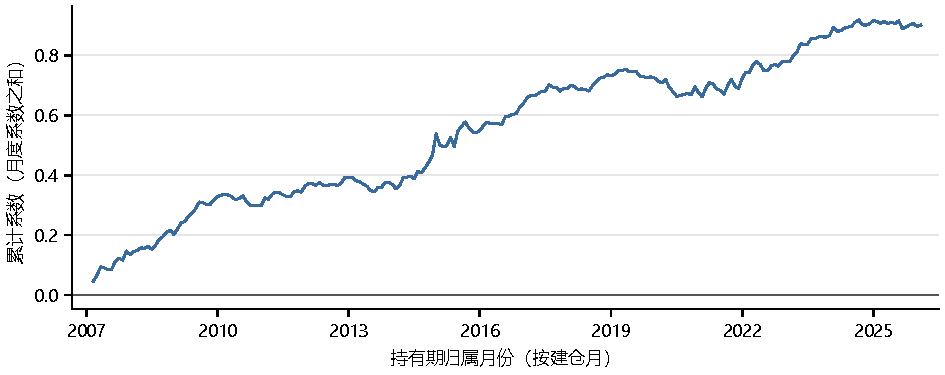
\includegraphics{figures/D3.pdf}
\caption*{\textbf{图D3　回归因子系数算术累计}\ 全部 A 股，228期；标准化BP的月度系数逐期相加，系数为小数，0.01对应1\%。横轴为持有期归属月份。}
\end{figure}

228期回归系数累计为0.9017，三个日历块分别贡献0.3690、0.3073、0.2253，正向累计分布在整个样本期。累计系数在2019-04达到0.7546后回落，2021-01降至最低（回落0.0929），2022-03创新高，低于前高34个月；2024-08以后至样本末端未再创新高（17个月）。同期累计Rank IC低于前高的区间都不超过7个月：2019年后线性斜率走弱，总体排序仍持续累积。

\Needspace{90mm}
\subsection{绝对净值、相对财富与滚动超额}
\begin{figure}[H]\centering
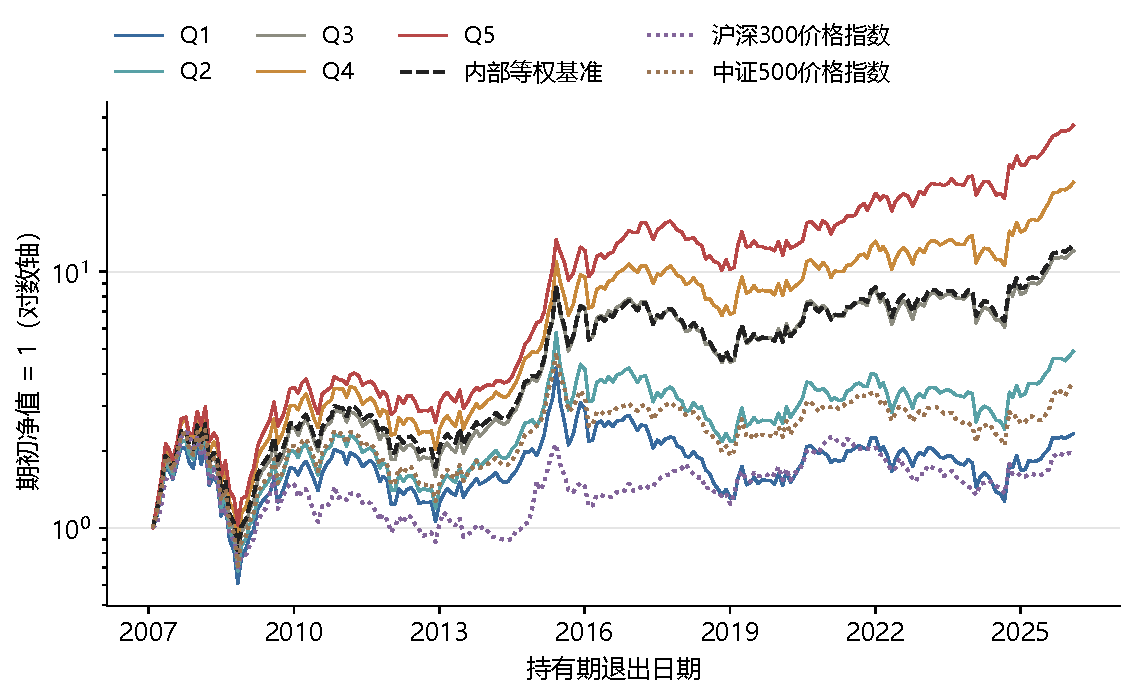
\includegraphics{figures/D4.pdf}
\caption*{\textbf{图D4　五层组合、内部基准与价格指数净值}\ 期初为1，实际端点2007-02-01至2026-02-02；纵轴为倍数，对数刻度；横轴为持有期归属月份。分层扣费，内部基准未扣费，外部价格指数不含分红。}
\end{figure}

同样从1开始，期末Q5净值为37.276，内部基准为12.739，Q1为2.330；沪深300和中证500价格指数分别为1.923与3.712。五层净值按层序拉开，Q5的期末财富约为内部基准的2.9倍、Q1的16倍；Q5期间最大回撤为$-$65.45\%。Q3与内部基准几乎重合（期末12.049与12.739）。

\Needspace{80mm}
\begin{figure}[H]\centering
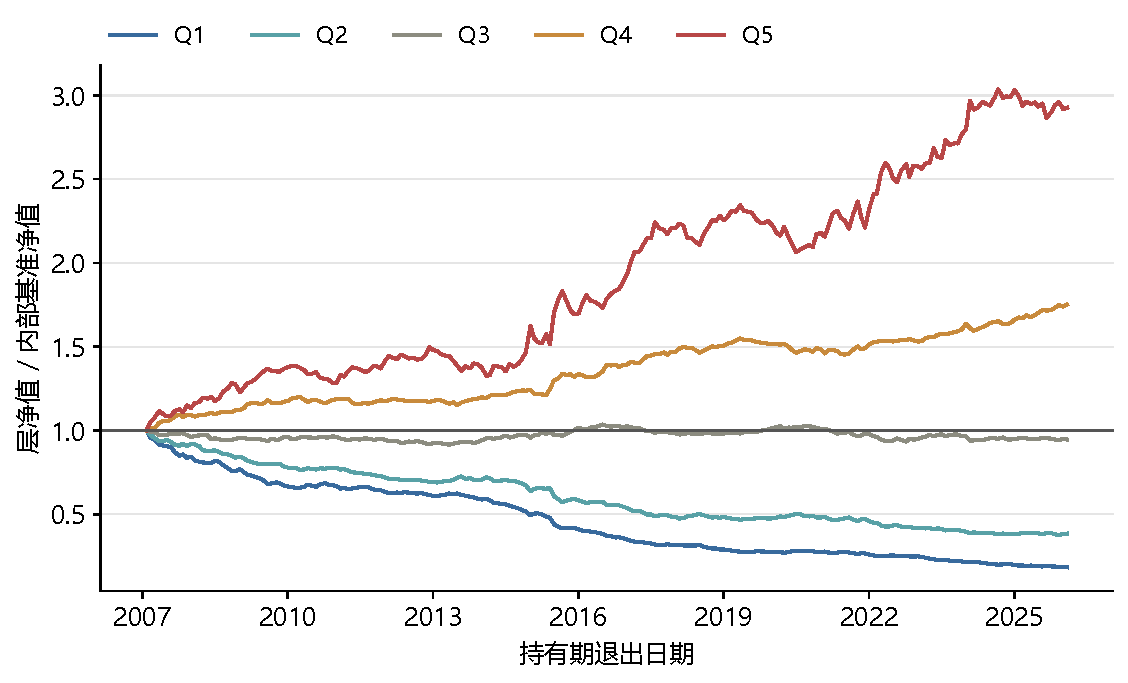
\includegraphics{figures/D5.pdf}
\caption*{\textbf{图D5　五层净值除以内部基准净值}\ 全部 A 股，228期；相对净值大于1表示截至当期的层净财富高于内部基准。阴影为Q5相对净值连续12个月以上低于此前高点的区间。}
\end{figure}

期末Q5/基准为2.926，Q4为1.751，Q3为0.946，各层相对财富按层序排列。Q5相对净值连续12个月以上低于此前高点的区间共六段（以下均计低于前高的观察月数）。最深的一段在2019-04见顶后回撤11.92\%（低点2020-06），2021-09创新高，期间28个观察月低于前高；其次是2012-11见顶后的24个月（最深$-$11.34\%）和2010-01见顶后的19个月（$-$7.37\%）；2015-08与2017-07见顶后另有12至13个月的较浅回撤（$-$7.54\%、$-$5.99\%）。2024-08见顶后的一段持续到样本末端，期末比前高低3.60\%。

\Needspace{90mm}
\begin{figure}[H]\centering
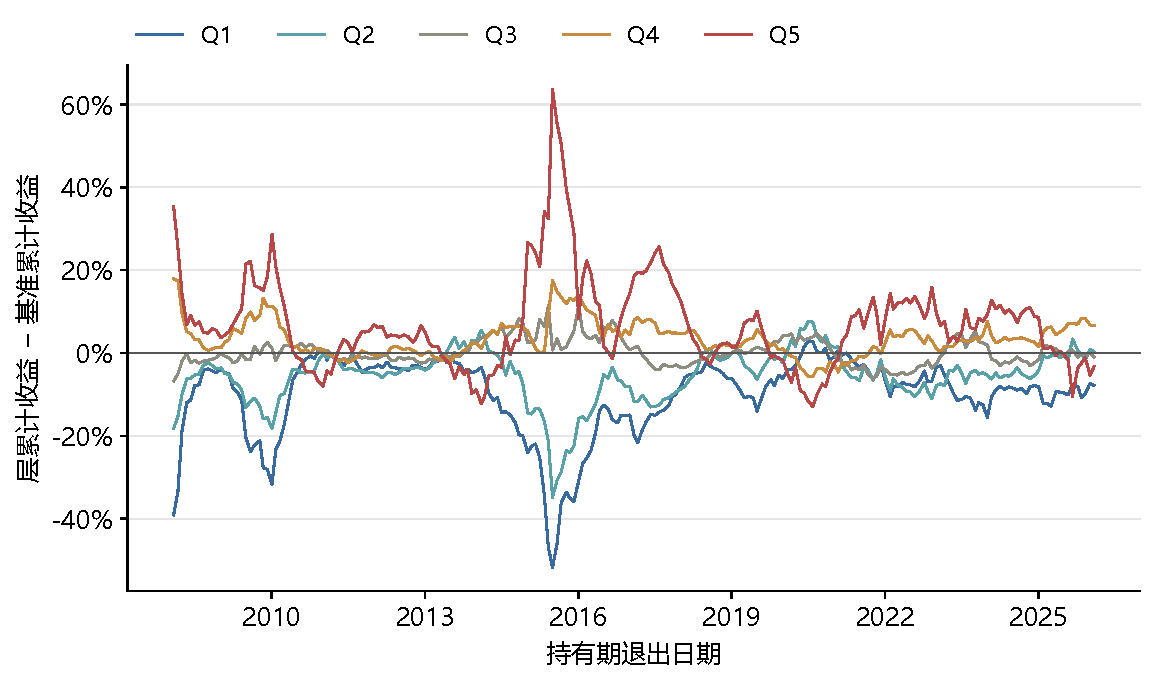
\includegraphics{figures/D6.pdf}
\caption*{\textbf{图D6　滚动12个月复利超额收益}\ 全部 A 股；层净收益复利减基准毛收益复利，纵轴以百分数显示差额；前11个月为空，共217个重叠窗口。阴影为Q5连续为负不少于6个端点的区间；横轴为窗口末月的持有期归属月份。}
\end{figure}

图D6把长期累计优势展开到具体窗口，分段均值见下表。

\begingroup\small\setlength{\tabcolsep}{4pt}
\begin{table}[H]\centering
\caption*{\textbf{表D6附表　各层滚动12个月超额的分段均值}}
\begin{tabular*}{\textwidth}{@{\extracolsep{\fill}}lrrrrrr@{}}\toprule
持有期归属区间 & 有效点 & Q1 & Q2 & Q3 & Q4 & Q5 \\ \midrule
2007-02至2013-12 & 72 & $-$7.75 & $-$5.12 & $-$0.71 & 2.57 & 5.08 \\
2014-01至2020-12 & 84 & $-$13.61 & $-$6.53 & 2.18 & 4.26 & 8.97 \\
2021-01至2026-01 & 61 & $-$7.80 & $-$4.69 & $-$1.36 & 3.19 & 6.55 \\
\bottomrule\end{tabular*}
\par\smallskip\raggedright\footnotesize 单位为百分点。分段按滚动端点归属，窗口可跨分段边界，相邻窗口重叠11期。\end{table}
\endgroup

Q5滚动超额为正的点为161/217（74.19\%）。按连续为负不少于6个端点的判据，失效区间有四段：2010-06至2011-03（10个端点，最低$-$7.99\%）、2013-04至2014-06（15个，$-$12.18\%）、2019-09至2021-01（17个，$-$12.91\%）和2025-06至2026-01（8个，$-$10.44\%）。最后一段持续到样本末端，末值为$-$3.26\%。三个分段的Q5均值均为正（5.08、8.97、6.55个百分点），五层分段均值也都按层序排列，失效期之外的超额足以弥补失效期的回落。

\Needspace{80mm}
\begin{figure}[H]\centering
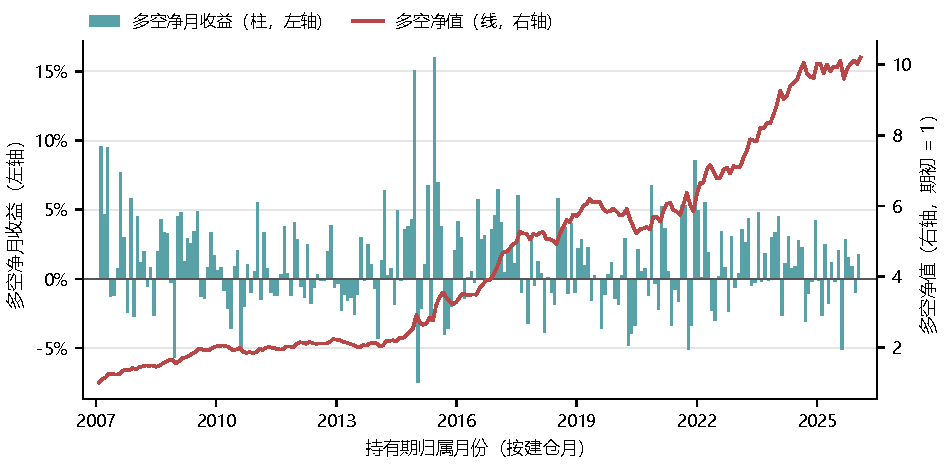
\includegraphics{figures/D7.pdf}
\caption*{\textbf{图D7　多空月收益与累计净值}\ 月收益读左轴，复利净值读右轴；Q5毛收益减Q1毛收益后扣两腿成本。两轴刻度相互独立；横轴为持有期归属月份。}
\end{figure}

多空正收益为136/228个月（59.65\%），期末净值10.197。最差月为2015-01（$-$7.49\%），最好月为2015-06（15.99\%），均按持有期起始月份归属。多空净值的最大回撤$-$15.66\%发生在2019-04至2020-06，2021-09回到前高，与D5、D6识别的失效期一致；此后至样本末端净值由6.194升至10.197。

\Needspace{80mm}
\subsection{五层与十层的风险调整表现}
\begin{figure}[H]\centering
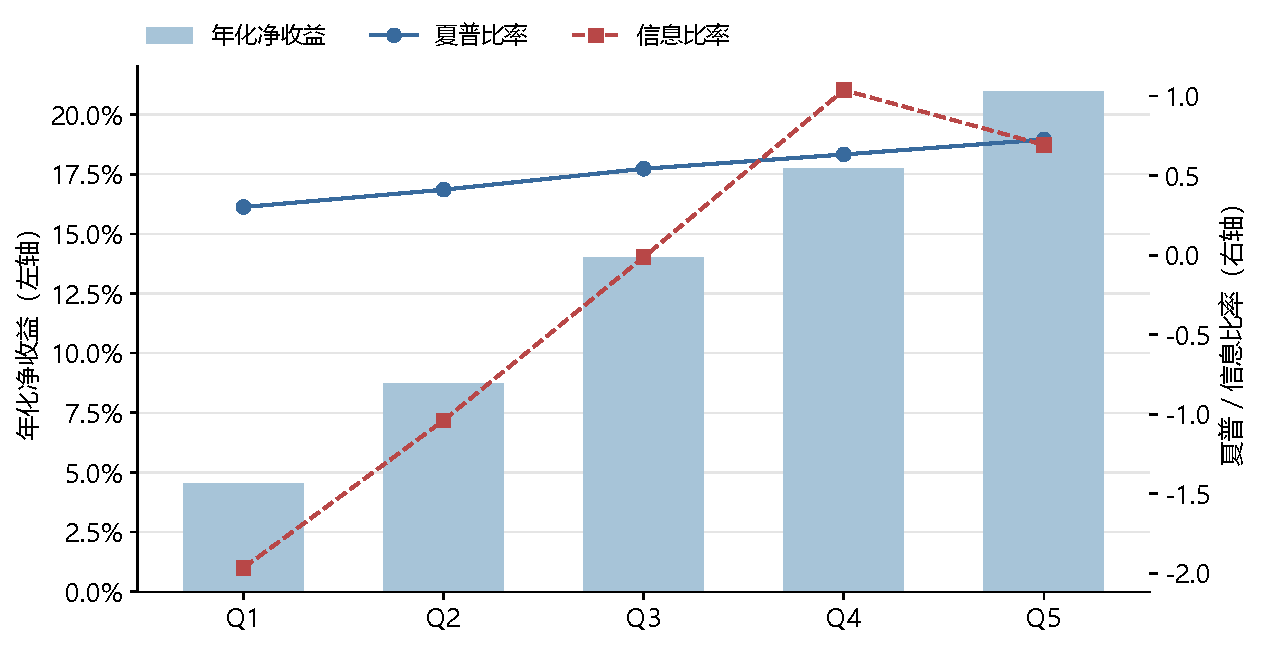
\includegraphics{figures/D8.pdf}
\caption*{\textbf{图D8　五层收益与风险调整指标}\ 年化净收益为柱，夏普与IR为双线；RF=0，时间序列标准差的分母为$n-1$；共228期。}
\end{figure}

五层年化净收益和夏普均逐层递增，Q5夏普为0.727。Q4的IR为1.038，高于Q5的0.693；相对月胜率分别为60.09\%和53.07\%（分母均为228期），超额最大回撤分别为$-$6.19\%和$-$11.92\%。Q5收益最高，Q4的信息比率最高、超额最大回撤最浅。

\Needspace{80mm}
\begin{figure}[H]\centering
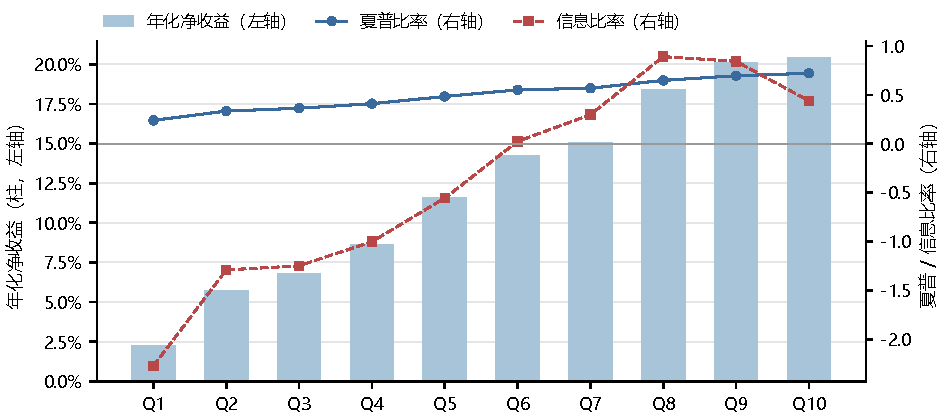
\includegraphics{figures/D9.pdf}
\caption*{\textbf{图D9　十层收益与风险调整指标}\ 保持全部 A 股样本、预处理及成本不变，只将五层改为十层；共228期。}
\end{figure}

十层年化净收益9/9对相邻层递增，层序秩相关1.000，单调性在更细分组下依然成立。Q9与Q10分别为20.12\%、20.43\%，最高尾部的收益增益已很小。Q10的算术年化超额为4.66个百分点，与Q9的4.92个百分点接近，但IR由0.843降至0.439，超额最大回撤由$-$9.21\%扩大到$-$17.61\%，相对月胜率由54.82\%降至49.12\%。最高中性化残差层的超额波动明显上升，与价值陷阱假说相容，但不能据此识别其成因。

\Needspace{80mm}
\subsection{流通市值三域}
\begin{figure}[H]\centering
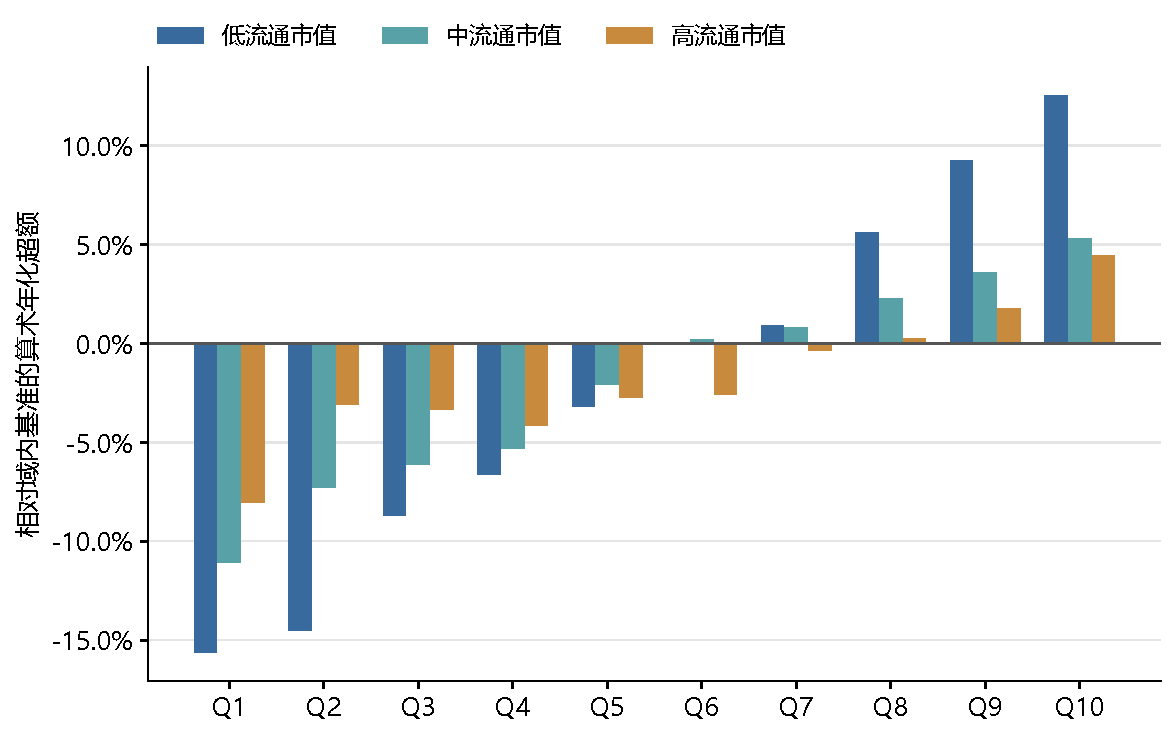
\includegraphics{figures/D10.pdf}
\caption*{\textbf{图D10　三市值域内十层年化超额}\ 各域先按流通市值形成，再按全部 A 股残差分层；年化超额为相对域内等权毛基准的算术年化超额。}
\end{figure}

低、中市值域的层序平滑，高市值域Q2至Q4出现倒序。附表列出域内股票数量、两端超额与Q10信息比率。

\begingroup\small\setlength{\tabcolsep}{4pt}
\begin{table}[H]\centering
\caption*{\textbf{表D10附表　市值域的样本量与两端超额}}
\begin{tabular*}{\textwidth}{@{\extracolsep{\fill}}lrrrrr@{}}\toprule
流通市值域 & 每期只数范围 & Q1年化超额 & Q10年化超额 & Q10信息比率 & 递增相邻层数/9 \\ \midrule
低 & 384--1755 & $-$15.64 & 12.54 & 0.905 & 9/9 \\
中 & 383--1755 & $-$11.08 & 5.31 & 0.622 & 9/9 \\
高 & 384--1755 & $-$8.03 & 4.44 & 0.387 & 7/9 \\
\bottomrule\end{tabular*}
\par\smallskip\raggedright\footnotesize 超额为相对域内基准（等权毛收益）的算术年化超额，单位为百分点；三域均有228期。每月先按流通市值三等分，再在各域内按同一份全部 A 股残差十等分。\end{table}
\endgroup

三域均有228期，Q10算术年化超额分别为12.54、5.31、4.44个百分点，信息比率为0.905、0.622、0.387；低、中市值域的十层超额均9/9递增，高市值域为7/9。BP的排序关系随市值上升而减弱，在低流通市值域最强。高市值域只有Q8至Q10为正超额，Q10信息比率不到低市值域的一半，大市值股票中的BP效应集中在最高几层。低市值域Q10建仓后平均月度只数换手约21.2\%，提示需关注成本影响，实际交易成本敏感性尚未评估。各域在BP及控制变量均有效的S样本中划分，因此域内BP完整率为100\%，不代表原始合格池的分域覆盖率；市值分界按每月等人数划分，先分域、再按全样本残差分层。

\clearpage
\subsection{一级行业内部比较}
\begingroup\small\setlength{\tabcolsep}{4pt}
\begin{longtable}{lrrrrrr}
\caption*{\textbf{表C4(a)　行业内五层的Q5绩效}}\\
\toprule
一级行业 & 有效期 & \makecell{年化超额\\（百分点）} & 夏普 & IR & \makecell{超额回撤\\（\%）} & \makecell{相对月\\胜率（\%）} \\ \midrule
\endfirsthead
\caption*{表C4(a)　行业内五层的Q5绩效（续）}\\\toprule
一级行业 & 有效期 & \makecell{年化超额\\（百分点）} & 夏普 & IR & \makecell{超额回撤\\（\%）} & \makecell{相对月\\胜率（\%）} \\ \midrule
\endhead
\midrule\multicolumn{7}{r}{续下页}\\\endfoot
\bottomrule\endlastfoot
家用电器 & 54/54 & 17.93 & 1.164 & 1.556 & $-$5.48 & 64.81 \\
美容护理 & 54/54 & 14.39 & 0.562 & 0.665 & $-$18.96 & 55.56 \\
电力设备 & 54/54 & 12.72 & 0.767 & 1.418 & $-$7.80 & 66.67 \\
食品饮料 & 54/54 & 10.59 & 0.555 & 1.276 & $-$4.64 & 61.11 \\
电子 & 54/54 & 10.01 & 0.824 & 1.084 & $-$7.42 & 57.41 \\
社会服务 & 54/54 & 9.84 & 0.887 & 0.874 & $-$8.34 & 61.11 \\
计算机 & 54/54 & 9.57 & 0.749 & 1.081 & $-$6.38 & 66.67 \\
医药生物 & 54/54 & 8.25 & 0.555 & 1.043 & $-$5.45 & 70.37 \\
农林牧渔 & 54/54 & 7.58 & 0.585 & 1.016 & $-$5.13 & 55.56 \\
纺织服饰 & 54/54 & 7.19 & 0.822 & 0.872 & $-$6.49 & 57.41 \\
交通运输 & 54/54 & 7.04 & 0.980 & 0.769 & $-$8.81 & 50.00 \\
非银金融 & 54/54 & 6.82 & 0.488 & 1.131 & $-$4.30 & 66.67 \\
机械设备 & 54/54 & 6.32 & 0.950 & 0.717 & $-$7.62 & 64.81 \\
国防军工 & 54/54 & 6.04 & 0.572 & 0.755 & $-$5.98 & 59.26 \\
公用事业 & 54/54 & 5.08 & 0.734 & 0.651 & $-$6.62 & 50.00 \\
石油石化 & 54/54 & 4.95 & 0.872 & 0.433 & $-$16.15 & 53.70 \\
银行 & 54/54 & 2.72 & 0.709 & 0.369 & $-$11.39 & 55.56 \\
环保 & 54/54 & 2.43 & 0.423 & 0.333 & $-$9.01 & 53.70 \\
有色金属 & 54/54 & 2.38 & 0.824 & 0.216 & $-$11.42 & 53.70 \\
汽车 & 54/54 & 2.07 & 0.798 & 0.191 & $-$16.61 & 51.85 \\
通信 & 54/54 & 1.60 & 0.896 & 0.162 & $-$15.17 & 55.56 \\
基础化工 & 54/54 & 1.45 & 0.562 & 0.189 & $-$9.65 & 53.70 \\
建筑装饰 & 54/54 & 0.80 & 0.645 & 0.072 & $-$18.77 & 48.15 \\
轻工制造 & 54/54 & 0.68 & 0.529 & 0.096 & $-$14.05 & 48.15 \\
传媒 & 54/54 & 0.52 & 0.765 & 0.038 & $-$16.68 & 53.70 \\
煤炭 & 54/54 & $-$0.09 & 0.527 & $-$0.006 & $-$24.71 & 48.15 \\
建筑材料 & 54/54 & $-$1.53 & 0.354 & $-$0.141 & $-$25.57 & 46.30 \\
商贸零售 & 54/54 & $-$4.69 & 0.440 & $-$0.626 & $-$17.40 & 42.59 \\
房地产 & 54/54 & $-$6.39 & 0.105 & $-$0.586 & $-$40.77 & 33.33 \\
钢铁 & 54/54 & $-$6.75 & 0.010 & $-$0.749 & $-$28.33 & 37.04 \\
综合 & 12/54 & --- & --- & --- & --- & --- \\
\end{longtable}
\noindent\footnotesize 共同信号窗为2021-07至2025-12（54期，持有期归属2021-08至2026-01），按年化超额降序。年化超额为算术年化超额；夏普对应Q5，IR、超额回撤和胜率相对行业内部基准（等权毛收益）。完整行业胜率分母均为54；综合行业不计算共同窗口绩效。\par
\endgroup

在2021-07至2025-12信号窗口（持有期归属2021-08至2026-01）的30个可比行业中，Q5年化超额为正25/30，BP在多数行业内有效。家用电器最高，为17.93个百分点；房地产与钢铁分别为$-$6.39和$-$6.75个百分点，商贸零售与建筑材料为$-$4.69和$-$1.53个百分点，煤炭接近零。综合行业未形成完整共同窗口，绩效留空。

\begingroup\small\setlength{\tabcolsep}{4pt}
\begin{longtable}{lrrlr}
\caption*{\textbf{表C4(b)　行业内收益排序与样本量}}\\
\toprule
一级行业 & \makecell{每期最少\\股票数} & \makecell{Q5收益\\名次} & 层收益排序 & 层序相关$\rho$ \\ \midrule
\endfirsthead
\caption*{表C4(b)　行业内收益排序与样本量（续）}\\\toprule
一级行业 & \makecell{每期最少\\股票数} & \makecell{Q5收益\\名次} & 层收益排序 & 层序相关$\rho$ \\ \midrule
\endhead
\midrule\multicolumn{5}{r}{续下页}\\\endfoot
\bottomrule\endlastfoot
家用电器 & 74 & 1 & $Q_5>Q_3>Q_4>Q_2>Q_1$ & 0.900 \\
美容护理 & 27 & 1 & $Q_5>Q_4>Q_2>Q_3>Q_1$ & 0.900 \\
电力设备 & 257 & 1 & $Q_5>Q_4>Q_3>Q_2>Q_1$ & 1.000 \\
食品饮料 & 105 & 1 & $Q_5>Q_4>Q_3>Q_2>Q_1$ & 1.000 \\
电子 & 317 & 1 & $Q_5>Q_4>Q_3>Q_2>Q_1$ & 1.000 \\
社会服务 & 65 & 1 & $Q_5>Q_4>Q_3>Q_2>Q_1$ & 1.000 \\
计算机 & 271 & 1 & $Q_5>Q_4>Q_3>Q_1>Q_2$ & 0.900 \\
医药生物 & 374 & 1 & $Q_5>Q_4>Q_3>Q_2>Q_1$ & 1.000 \\
农林牧渔 & 87 & 1 & $Q_5>Q_4>Q_2>Q_3>Q_1$ & 0.900 \\
纺织服饰 & 98 & 1 & $Q_5>Q_4>Q_2>Q_3>Q_1$ & 0.900 \\
交通运输 & 120 & 1 & $Q_5>Q_3>Q_4>Q_2>Q_1$ & 0.900 \\
非银金融 & 77 & 1 & $Q_5>Q_4>Q_2>Q_3>Q_1$ & 0.900 \\
机械设备 & 418 & 1 & $Q_5>Q_4>Q_3>Q_2>Q_1$ & 1.000 \\
国防军工 & 108 & 1 & $Q_5>Q_4>Q_3>Q_2>Q_1$ & 1.000 \\
公用事业 & 112 & 1 & $Q_5>Q_4>Q_3>Q_2>Q_1$ & 1.000 \\
石油石化 & 42 & 1 & $Q_5>Q_2>Q_3>Q_1>Q_4$ & 0.300 \\
银行 & 40 & 1 & $Q_5>Q_3>Q_4>Q_1>Q_2$ & 0.800 \\
环保 & 103 & 1 & $Q_5>Q_4>Q_3>Q_2>Q_1$ & 1.000 \\
有色金属 & 118 & 2 & $Q_3>Q_5>Q_2>Q_4>Q_1$ & 0.500 \\
汽车 & 217 & 2 & $Q_3>Q_5>Q_4>Q_2>Q_1$ & 0.700 \\
通信 & 98 & 1 & $Q_5>Q_4>Q_3>Q_1>Q_2$ & 0.900 \\
基础化工 & 311 & 2 & $Q_4>Q_5>Q_3>Q_2>Q_1$ & 0.900 \\
建筑装饰 & 134 & 3 & $Q_4>Q_3>Q_5>Q_2>Q_1$ & 0.700 \\
轻工制造 & 122 & 2 & $Q_4>Q_5>Q_2>Q_3>Q_1$ & 0.800 \\
传媒 & 120 & 2 & $Q_4>Q_5>Q_2>Q_3>Q_1$ & 0.800 \\
煤炭 & 33 & 3 & $Q_1>Q_4>Q_5>Q_2>Q_3$ & -0.200 \\
建筑材料 & 72 & 3 & $Q_4>Q_3>Q_5>Q_1>Q_2$ & 0.600 \\
商贸零售 & 90 & 4 & $Q_3>Q_4>Q_2>Q_5>Q_1$ & 0.300 \\
房地产 & 88 & 5 & $Q_3>Q_4>Q_2>Q_1>Q_5$ & -0.100 \\
钢铁 & 43 & 4 & $Q_3>Q_4>Q_1>Q_5>Q_2$ & 0.100 \\
综合 & 15 & --- & 样本不足 & --- \\
\end{longtable}
\noindent\footnotesize 收益排序按各层年化净收益从高到低排列；相关系数是层序与年化收益的Spearman相关。共30个完整行业，综合行业保留不足行。\par
\endgroup

Q5在19/30个可比行业排名第一，在24/30个行业进入前二，行业内排序整体稳健。层序方向相反的行业为煤炭（$\rho=-0.200$，Q1收益最高）和房地产（$\rho=-0.100$，Q5收益最低）；商贸零售与钢铁的Q5名次为第4。石油石化Q5虽排名第一，层序相关只有0.300。美容护理每期最少仅27只，接近25只门槛。综合行业只有12/54期达到门槛，列为样本不足。
